\documentclass[a4paper,12pt]{kth-mag}
\usepackage[T1]{fontenc}
\usepackage{textcomp}
\usepackage{lmodern}
\usepackage[utf8x]{inputenc}
\usepackage[swedish,english]{babel}
\usepackage{modifications}
\usepackage{minted}
\usepackage{cite}
%\usepackage{float}
% IMPORTANT! This need to be the last package loaded since it overwrites features from others to work correctly
\usepackage[pdfusetitle=true, pdfauthor={Pascal Chatterje and Joakim Carselind}, pdfsubject={Bachelors essay 2012 (dkand12) in computer science and communication at Royal Institute of Technology, Stockholm, Sweden}, pdfkeywords={Concurreny,JVM,Java,Groovy,Clojure}, pdftex]{hyperref}

\definecolor{code}{rgb}{0.95,0.95,0.95}

\title{Concurrency on the JVM}

\subtitle{An investigation of strategies for handling concurrency in Java, Clojure and Groovy}
          
\foreigntitle{En undersökning av strategier för hantering av parallellism i Java, Clojure och Groovy}
              
\author{Pascal Chatterjee \and Joakim Carselind \\ \small{\{pascalc, joacar\}@kth.se}}
\date{April 2012}

\blurb{Bachelor's Thesis at NADA\\Supervisor: Mads Dam\\Examiner: Mårten Björkman}
\trita{TRITA xxx yyyy-nn}

% Magic
\makeatletter\@addtoreset{section}{part}\makeatother%
\renewcommand{\thesection}{\arabic{section}}

\begin{document}

\frontmatter
\pagestyle{empty}
\removepagenumbers
\maketitle
\selectlanguage{english}

\begin{abstract}
    Processors with multiple cores opens up for better utilisation of hardware resources for applications if they take advantage of concurrency and parallelism. There are several methods to reap the benefits of concurrency; software transactional memory, actors and agents, locks and threads. The use of parallelism in programming comes at a price: synchronisation between threads operating on shared memory resources.

New software libraries and programming language exists to simplify implementation of parallel application and this essay investigate strategies on those with the Java Virtual Machine as a commonon denominator: Java, Clojure and Groovy.
\endinput
\end{abstract}

\clearpage

\begin{foreignabstract}{swedish}
  Flerkärniga processorer skapar grund för bättre nyttjande av hårdvaruresurser för applikationer implementerade parallelt. Det existerar ett flertal methoder för att skörda fördelarna av parallelism: software transactional memory, skådespelare och agenter, lås och trådar. Men parallelism har ett pris: att synkronisera trådarna som arbetar på delade minnesresurser.

Nya mjukvarubibliotek och programeringsspråk existerar för att förenkla implementationen av parallella applikationer och i denna uppsats undersöker vi de som har en gemensam nämnare Javas virtuella maskin: Java, Clojure och Grooy. 
\endinput
\end{foreignabstract}

\clearpage
\section{Statement of collaboration}
hejhopp

\clearpage

\tableofcontents*
\mainmatter
\pagestyle{newchap}
\makeatletter\@openrightfalse

\chapter{Introduction}
More cores let the computer execute instructions like add or move parallel which could increase the performance of a software application. However, the potential performance gain comes with a price namely increased control over synchronisation to prevent memory corruption in shared memory resources. Since traditional sequential execution is, to some extent, abandoned for concurrent execution, a situation arise that could cause the application to behave non-deterministically.

For this reason, synchronisation plays a crucial role to maintain consistency and correctness in concurrent environments.

The type\footnote{In the aspect of read and write operations or computationally intense} of the application has a significant role when parallel computing is an alternative. The frequency and distribution of opertions is to be taken into account when the architecture is sketched and the solution designed. Applications that consists of mutually exclusive operations such as distributed database queries performs well under concurrency whilst applications tackling a computationally hard problem see no or insignificant performance gain when implemented with a parallel design.

Modern, dynamic languages like Ruby and Python feature a \textit{Global Interpreter Lock} (GIL), so we need to use languages such as C/C++/Java to leverage multiple processors. We will focus on the JVM in this paper.

\part{Introducing concurrency}

\section{Concurrency control} \label{sec:con_con}
Concurrency control defines guidelines to maintain data integrity and achieve correctness in concurrent environments such as hardware modules and operating systems\cite{concon}. When modules, regarding level, communicates concurrently there is a risk of the data integrity being violated. The consequence could be that the system stop working or, even worse, continue working without exception. If situations like this occurs, they may be extremely difficult to reproduce and debug. Therefore the use of concurrency control is highly important to make sure that the system conforms to rules applicable for concurrent environments.

\section{Threads}
A thread is a light weight process with low inter-thread communication overhead. The low utilisation of resources inside the process and low communication overhead is beneficial for an application leveraging concurrency. 

The existens of multiple threads inside a process brings up a risk of different threads operating on the same memory resource and due to this synchronisation is important to maintain correctnes in the program. The operations performed by threads \textit{need} to be \textbf{atomic} if they execute code in a \textbf{critical section} in the context of the process memory and shared mutuable resources.

\section{Atomicity}

One of the first things we should realise when writing concurrent programs is that most of the statements we use are not \textbf{atomic}. This means that although we tend to think of them as indivisible units of computation, they expand to multiple instructions when compiled to bytecode. It is these instructions that are atomic, not the statements we write in high-level JVM languages.

Let us take the simple example of incrementing an integer variable. In Java, we could write the function:

\begin{listing}[H]
\begin{minted}[linenos=true,bgcolor=code]{java}
public static void add(int var, int num) { 
	var = var + num; 
}
\end{minted}
\end{listing}

Intuitively, we might think that that if a context switch were to occur in our function, it would take place at line 1, 2 or 3. This would be the case if line 2 was atomic, but as it consists of addition \textit{and} assignment, it is compiled to multiple bytecode instructions. We can see these instructions here:

\begin{listing}[H]
	\begin{minted}[linenos=true,bgcolor=code]{java}
public static void add(int, int);
	iload_0
	iload_1
	iadd
	istore_0
	return
  	\end{minted}
\end{listing}

The second line from our Java \texttt{add} function generates the \texttt{iadd} and \texttt{istore0} instructions at lines 4 and 5 of the bytecode. 

It is entirely possible for a thread switch to occur in between these instructions. Usually this is not problematic at all, and in fact this happens many times a second on all modern operating systems. However, if multiple threads attempt to change the value of the \textit{same} variable at the same time, inconsistencies begin to arise. 

\section{Shared memory}

In order to better illustrate the lack of atomicity in our add function, we can rewrite it to look like this:

\begin{listing}[H]
	\begin{minted}[linenos=true,bgcolor=code]{java}
public static void add(int num) 
throws InterruptedException {
        int v = var;
        Thread.sleep(1);
        var = v + num;
}
  	\end{minted}
\end{listing}

Here \texttt{var} is an instance variable. The \texttt{Thread.sleep} at line 4 forces a context switch after \texttt{var} has been copied to the local variable \texttt{v}. If any other thread alters \texttt{var} during this time, those changes will be lost when the original thread resumes and writes \texttt{v + num} back to \texttt{var}. The following could well happen if two threads were to execute \texttt{add} simultaneously:

\begin{listing}[H]
	\begin{minted}[linenos=true,bgcolor=code]{java}
   // var = 0
   // Thread 1
    int v = var; // v = 0
    Thread.sleep(1);
    // * Context Switch *
        // Thread 2
        int v = var // v = 0
        Thread.sleep(1)
        var = v + 1 // var = 1
        // * Context Switch *
    var = v + 1; // var = 1
  	\end{minted}
\end{listing}

As we can see, after this interleaving of statements, \texttt{var = 1} even though it was incremented \textit{twice}. It is in this way that shared mutable memory, or state, can lead to inconsistent data even though the program logic is correct. We call this phenomenon - when the result of a program is dependent on the sequence or timing of other events - a \textbf{race condition}.

\begin{figure}[H]
\begin{center}
    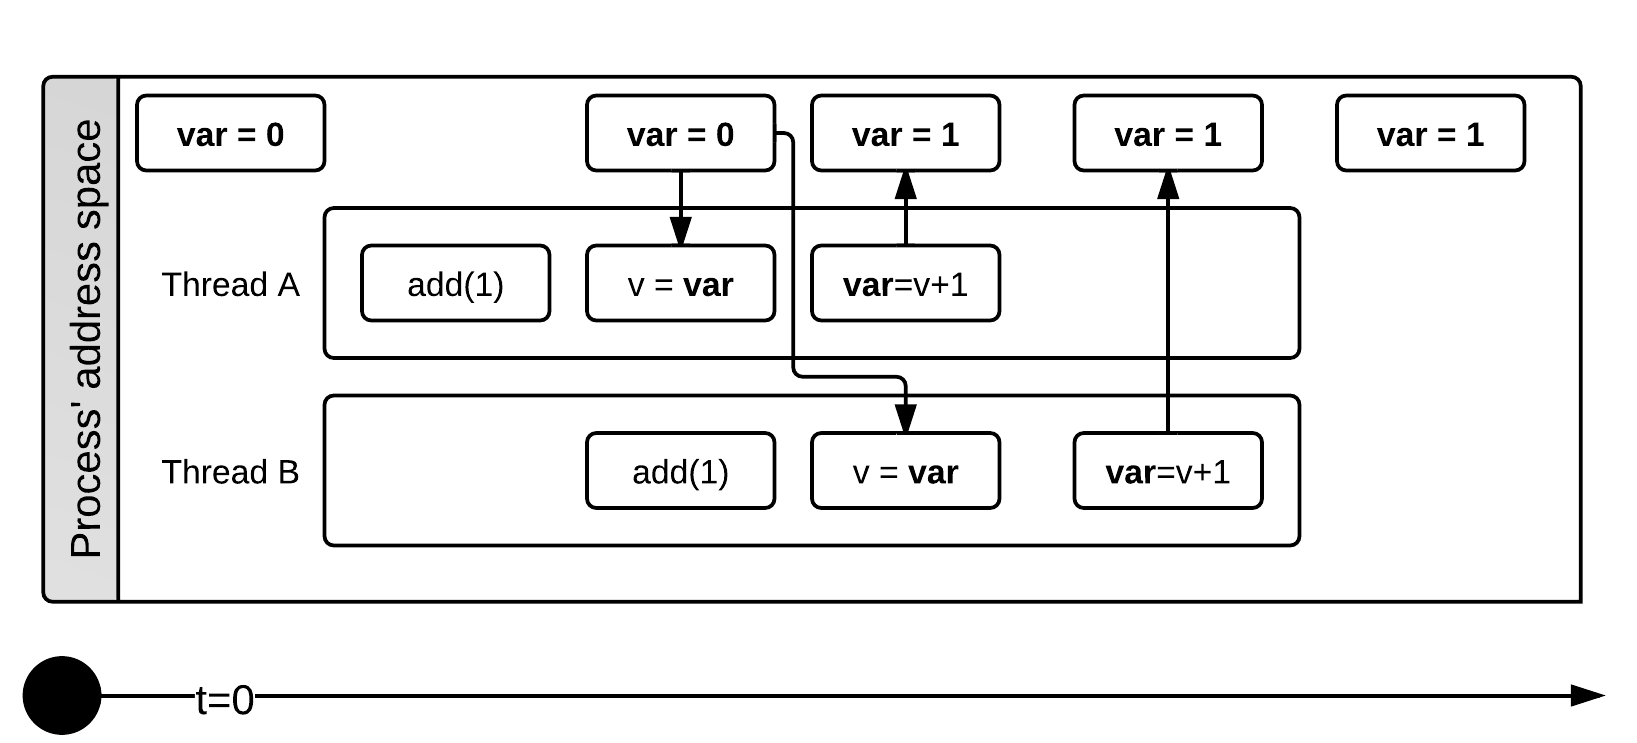
\includegraphics{images/ProcessAndThreads.png}
\caption{Process and threads synchronisation issue.}\label{fig:pat_sync_issue}
\end{center}
\end{figure}

All of the concurrency strategies we will discuss in this paper aim to mitigate the effects of race conditions, and thereby ensure that programs behave in a deterministic way despite the activity of multiple threads. They do this by eliminating one of the factors from \textbf{uncontrolled access to shared, mutable state} that can lead to problems. The first approach we consider, threads and locks, uses locks to \textbf{control access} to shared mutable state.

\part{Threads and Locks}

\section{Background}
When an application is initiated from the operating system, a process is created to host the application and the process define the address space allocated in the primary memory (random access memory). 

Typically there are many processes running simultaneously and each process can have multiple threads. A thread performs small tasks for the process and has low overhead for inter-thread communication in contrast to inter-process communication. The low communication overhead is advantageous for parallelism since a process has a well defined address space, threads leap a high risk executing overlapping operations on the same resource, the synchronisation of the resources is crucial.

We will use the example of bank accounts that allow withdrawals, deposits and reading the value of a balance to illustrate the concurrency strategies in this paper. Formally we can view this as an interface, that in Java can be written:

\begin{listing}[H]
	\begin{minted}[linenos=true,bgcolor=code]{java}
public interface Account {
    public float getBalance();
    public boolean deposit(float amount);
    public boolean withdraw(float amount);
}
  	\end{minted}
\end{listing}

\texttt{getBalance} returns the current balance as a \texttt{float}; \texttt{deposit} and \texttt{withdraw} increment and decrement the current balance respectively, and return a boolean signifying whether they succeeded. \texttt{withdraw} can fail if more funds are requested than are present in the balance.

\newpage

\section{No locks}

We begin by implementing the \texttt{Account} interface in the simplest possible way.

\begin{listing}[H]
	\begin{minted}[linenos=true,bgcolor=code]{java}
public class NaiveAccount implements Account {
    private float balance = 0;

    public float getBalance() {
    		Thread.sleep(1);
        return balance;
    }

    public void deposit(float amount) 
    throws InterruptedException {
        float b = balance;
        Thread.sleep(1);
        balance = b + amount;
    }

    public void withdraw(float amount) 
    throws InterruptedException {
        float b = balance;
        Thread.sleep(1);
        balance = b - amount;
    }
}  
	\end{minted}
\end{listing}

As we explained in section 1.3, we insert a \texttt{Thread.sleep} in the middle of \texttt{deposit} and \texttt{withdraw} in order to highlight the danger of context switches.

\subsection{Testing correctness}

We can (informally) test the correctness of this implementation by initially depositing a certain amount in an account, carrying out a certain number of deposits and withdrawals, and then making sure that the resulting balance is as we expected.

In these tests the initial balance is \texttt{10}, and we carry out a sequence of 10 deposits and 10 withdrawals, each for the amount of \texttt{1} unit. As these cancel out, our finishing balance should also be \texttt{10} as that is what we started with. These operations are themselves carried out 10 times to see what happens when they are repeated.

\subsubsection{Single Threaded}

The collected final balances of the single threaded tests are shown below:

\begin{listing}[H]
	\begin{minted}[bgcolor=code]{java}
[10.0, 10.0, 10.0, 10.0, 10.0, 10.0, 10.0, 10.0, 10.0, 10.0]
	\end{minted}
\end{listing}

As we can see, these final balances are exactly what we would expect given an initial balance of 10, followed by 10 deposits and 10 withdrawals of 1 unit. The results were also unchanged over the course of 10 trials.

\subsubsection{Multiple Threaded}

Now let's see what happens when we run the withdrawals and the deposits in separate threads. 

\begin{listing}[H]
	\begin{minted}[bgcolor=code]{java}
[8.0, 20.0, 20.0, 20.0, 6.0, 0.0, 16.0, 18.0, 8.0, 0.0]
	\end{minted}
\end{listing}

Here the final balance ranged between 0 and 20, which is an error of $-10 \leq error \leq 10$. This shows that in some runs all our withdrawals disappeared; in others all our deposits disappeared; and sometimes we saw a mixture of these two extremes. Such disappearances of actions from our results happened when a certain interleaving of statements from the two threads occurred as described in section 1.3.

\begin{table}[h]
    \centering
    \begin{tabular}{lc}    
    \textbf{Mean} & 11.6 \\
    \textbf{Deviation} & 7.2 \\ 
    \end{tabular}
\end{table}

This makes it very obvious that the \texttt{deposit} and \texttt{withdraw} methods are \textbf{critical sections} - a section of code that should only be executed by one thread at any time. These sections need to be \textbf{mutually exclusive} so that we can reason about their effects as if they were atomic actions. Our problems arise only when a thread context switches while leaving the shared, mutable balance variable in an inconsistent state. 

\section{Locking with \texttt{synchronized}}

Our first solution to this problem will be to use Java's \texttt{synchronized} concept to ensure that even if a context switch occurs within a critical section, other threads are blocked from entering until the currently executing thread completes its actions.

The changes to the code to facilitate this are minimal: we simply insert the keyword \texttt{synchronized} into the signature of any method that references the shared variable \texttt{balance}. For us, this is all three methods (even \texttt{getBalance} which should not be allowed access to \texttt{balance} during a \texttt{deposit} or \texttt{withdraw} as it is by definition inconsistent at that time).

\subsection{Testing correctness}

Running the multi-threaded test, with simultaneous deposits and withdrawals, yields the results:

\begin{listing}[H]
	\begin{minted}[bgcolor=code]{java}
[10.0, 10.0, 10.0, 10.0, 10.0, 10.0, 10.0, 10.0, 10.0, 10.0] 
	\end{minted}
\end{listing}

Our problems seem to be solved! Unfortunately, this form of overzealous locking suffers from some performance issues which we will discuss next.

\subsection{Performance}

Threads attempting to enter \texttt{synchronized} methods have to acquire an object's intrinsic lock, or \textbf{monitor}, before they can execute any code\footnote{http://docs.oracle.com/javase/tutorial/essential/concurrency/syncmeth.html}. This ensures that all \texttt{synchronized} methods are mutually exclusive, which is good for our \texttt{deposit} and \texttt{withdraw} operations, but can be wastfeul for \texttt{getBalance}. The difference, of course, is that \texttt{deposit} and \texttt{withdraw} are mutators whereas \texttt{getBalance} is simply an accessor, and while mutators should mutually exclude all other operations, there is no reason why accessors should exclude other accessors as they do not change the state of an object. 

We can see the performance implications of this by carrying out a test in which 9 threads execute \texttt{getBalance} and 1 thread executes \texttt{deposit} in parallel. If this test takes around the same time to complete as the inverse, where 9 threads execute \texttt{deposit} and 1 thread executes \texttt{getBalance}, then we can conclude that accessors and mutators are all mutually exclusive.

\begin{listing}[H]
	\begin{minted}[bgcolor=code]{java}
Synchronized Read Frenzy: 121.0 ms
Synchronized Write Frenzy: 124.0 ms
	\end{minted}
\end{listing}

As there is no perceptible difference between the read frenzy, with more reads than writes, and the write frenzy, with the inverse, we can conclude that both reads and writes have been serialised by the object's monitor which we invoked using \texttt{synchronized}.

\section{Explicit locks}

Luckily for us, Java has included support for more finely-grained locks than an object's monitor since version 1.5. Of these, the \texttt{ReentrantReadWriteLock} is most suitable for our purposes. This object actually consists of two locks, a read-lock and a write-lock. The write-lock, like the object's monitor, mutually excludes everything. The read-lock however, allows multiple threads to acquire it at the same time, but still excludes other threads from acquiring the write-lock.

This has the effect of allowing read operations to execute in parallel while serialising writes. The reentrant part of the lock's name signifies that either lock may be acquired multiple times - such as read methods calling other read methods, with no ill effects.

An implementation of a \texttt{ReadWriteLockAccount} is as follows:

 \begin{listing}[H]
	\begin{minted}[linenos=true,bgcolor=code]{java}
public class ReadWriteLockAccount implements Account {
    private float balance = 0;
    private final ReentrantReadWriteLock rwl = 
    		new ReentrantReadWriteLock();
    private final Lock readLock = rwl.readLock();
    private final Lock writeLock = rwl.writeLock();

    public float getBalance() 
    throws InterruptedException {
        readLock.lock();
        try { 
            Thread.sleep(1);
            return balance; 
        }
        finally { readLock.unlock(); }
    }

    public boolean deposit(float amount) 
    throws InterruptedException {
        writeLock.lock();
        try {
            float b = balance;
            Thread.sleep(1);
            balance = b + amount;    
            return true;
        } finally { writeLock.unlock(); }
    }

    public boolean withdraw(float amount)
    throws InterruptedException {
        writeLock.lock();
        try {
            if (balance - amount >= 0) {
                float b = balance;
                Thread.sleep(1);
                balance = b - amount;
                return true;
            } else { return false; }
        } finally { writeLock.unlock(); }
    }
}
	\end{minted}
\end{listing}

\subsection{Performance}

Let's see how this Account performs during read and write frenzies.

\begin{listing}[H]
	\begin{minted}[bgcolor=code]{java}
Read-Write-Lock Read Frenzy: 26.0 ms
Read-Write-Lock Write Frenzy: 123.0 ms
	\end{minted}
\end{listing}

Now that read operations such as \texttt{getBalance} can execute in parallel, the read frenzy test is significantly faster than the write frenzy, in which no parallelisation is possible. Also worth noting is that the write frenzy here took around the same time as our \texttt{synchronized} version. This shows that using a \texttt{ReadWriteLock} should usually yield \textit{at least as good} performance as the \texttt{synchronized} keyword, with performance during heavy read activity receiving the most benefits and heavy write activity staying the same.

\subsection{Boilerplate code}

One area in which the \texttt{synchronized} Account beats the \texttt{ReadWriteLock} version is in the amount of boilerplate code that is required to maintain correctness. The \texttt{synchronized} Account required only three extra words compared to our original Account, whereas our latest version requires explicit locking and unlocking of specific locks to surround the body of each critical method. 

In our example this is not so bad, especially considering the increased performance these locks have given us, but in larger projects the amount of code-overhead introduced by explicit locking can be significant. In fact, code which includes overhead like this is harder to parse (as a programmer), maintain, and is also more fragile, as forgetting to unlock in just one place can introduce severe bugs into a system.

More flexible languages than Java combat this problem by using macros and higher-order functions to abstract away such boilerplate code, as we will see in later sections.

\section{Transfers}

Now that we have a correct and performant Account implementation, our job seems to be done. As before, things are not quite so simple. Our latest Account implementation appears to work in isolation, but things can get trickier when we bring multiple Accounts into the mix.

Let us imagine that we want to transfer funds between Accounts. A \texttt{transfer} method could be defined in some sort of \texttt{AccountTransferService} class, which would take 2 Accounts and an amount as input, withdraw \texttt{amount} from the first Account, and then deposit \texttt{amount} in the second Account. These \texttt{transfer}s are also critical sections, as Accounts should not be altered or read mid-transfer as they are in an inconsistent state.

To ensure the integrity of this critical section we have to acquire locks on both Accounts, carry out the transfer, and then release the lock. The object monitor version is shown below (an explicit lock version would acquire the objects' write-locks instead):

\begin{listing}[H]
	\begin{minted}[linenos=true,bgcolor=code]{java}
public static void transfer(Account from, Account to,
float amount) throws InterruptedException {
        synchronized(from) {
            Thread.sleep(1);
            synchronized(to) {
                from.withdraw(amount);
                to.deposit(amount);
            }
        }
    }
	\end{minted}
\end{listing}

This code will work as expected the vast majority of the time, but there is a case in which not only will the program be incorrect, it will actually hang forever. As you can imagine, this is because of the inconveniently placed \texttt{Thread.sleep} on line 4. 

Like before, this line forces a context switch that could occur in the normal execution of the code. This is usually not a problem, except for the case in which a transfer \textbf{from} Account A \textbf{to} Account B, and a transfer \textbf{from} Account B \textbf{to} Account A occur simultaneously. This will result in the following sequence of events:

\begin{enumerate}
\item Transfer 1: Acquires Account A's lock
\item Context switch
\item Transfer 2: Acquires Account B's lock
\item Transfer 1 waits to acquire Account B's lock
\item Transfer 2 waits to acquire Account A's lock
\end{enumerate}

As both transfers are waiting for each other, their threads will block indefinitely in a situation known as \textbf{deadlock}.

This dangerous juggling of locks is possibly the greatest problem that arises when using Threads and Locks to manage concurrency. Other concurrency strategies like the ones we will discuss later abstract away the handling of locks, meaning that it is much harder to make mistakes involving them.

\section{Composability / Reuse}

Removing context-specific locking code also enhances the composability of a system and encourages code reuse etc etc.

\part{ Actors}

\section{Background}
When using object-oriented programming (OOP), encapsulation of an objects data is of uttermost importance to maintain its internal data integrity. Via instance methods the state of the object can be changed and whilst this work well in a single-threaded environment it fails in multi-threaded environments. Multiple threads might call the instance methods concurrently and jeopordize isolation and consistency. 

Actors provide well definied states, where transition to another and behaviour is determined by receiving a message which is communicated asychronously. These messages could be an \texttt{Integer}, a \texttt{String} or even a \texttt{Class} if immutable. Upon receiving a message an actor respond in one, or more, ways\cite{scalaactors}
\begin{enumerate}
 \item Send out messages to known actors, it self included
 \item Change state and hence behaviour when receiving next message
 \item Create more actors
\end{enumerate}
Above mentioned is typical charateristics of an event-based program and to some extend actors could be viewed as event-based.

\section{A naive version}
account sim.groovy -> deadlock.
\section{Introducing brokers}
\section{Active Objects}
\subsection{Inheritance}
\subsection{Code reuse}
\subsection{Problems}
transfer is a ''fake'' transaction.

\part{ Software Transactional Memory}

\section{Background}
Software transactional memory (STM) is influenced by database transactions and that operations are conceptually \textbf{atomic}. STM provides abstraction of handling in-code synchronisation and provide the appearence that code is executed sequentially. Every transaction maintains a log to track its progress in case it would be \textit{aborted} to enable the operations to be \textit{rollbacked}. If the transaction was successful the operations is \textit{commited} and changes made permanent.

The use of operations with side effects in transactions is highly discouraged due to difficulties to perform rollback. For example I/O-operations could prove extremely hard to redo and printing to, e.g. a log, could obfuscate the log. Best practice is to schedule operations with side effects in a post-commit section.

STM enables composition of atomic operations\cite{cmt} which is not possible to achieve in tradtional lock-based programs. This prove extremely useful when altering high-level data structures, e.g. hash tables, by composing atomic operations such as \texttt{delete} and \texttt{insert} to be executed sequentially. 

\section{Concurrency in Clojure}
Clojure provides a separation of value and identity, where an identity could be viewed as time keeper and the values are the previous values, i.e. time that has passed. As time pass, old values (value) are added to a history record, but the time keeper (identity) remains intact and change state to its current time (value). Since the history records consists of just that, history, they are immutable: what has happened has happened. In Clojure all values and structures are, by design, \textbf{immutable} (see Section~\ref{sec:immutability}) and an identity is only subject for mutability inside a \textbf{transaction} (see Section~\ref{sec:transactions}).

To take advantage of STM transactions in Clojure, one must use immutable and \textbf{persistent} data structures\cite{sub11}. Appropriately enough, this is the case for \textit{all} data structures in Clojure. The use of persisitent and immutable data structures combined with separation of values and identity creates a high performing concurrency environment\footnote{Highest performance is achieved in environments with high-read and low-write that implies low collision frequency.} without the need of lock-based programming.

For example, if multiple threads work on different accounts, then there is no need for synchronisation. But as soon as two transactions attempt to modify a shared resource, the \textbf{transaction manager} steps in to ensure consistency and correctnes. After the transaction has completed, the old value will quietly be removed by the garbage collector since there is no reference pointing towards it.

In Clojure the \texttt{dosync} does the trick to ensure consistency and integrity. The code blocks wrapped in the \texttt{dosync} context is ensured to use correct transaction methodology when altering a value. Lets look at the code:
\begin{listing}[H]
    \begin{minted}[linenos=true,bgcolor=code]{clojure}
; Account manipulation functions
(defn get-balance [balance]
    (dosync
        (. Thread sleep 1)
        @balance))

(defn insert [balance amount]
    (dosync
        (. Thread sleep 1)
        (alter balance + amount)))

(defn withdraw [balance amount]
    (dosync
        (. Thread sleep 1)
        (alter balance - amount)))

(defn transfer [balance1 balance2 amount]
    (dosync
        (withdraw balance1 amount)
        (. Thread sleep 1)
        (insert balance2 amount)))
    \end{minted}
\end{listing}
If any thread attempts to do an \texttt{insert} ''behind the back'' (from the transactions perspective) during an ongoing \texttt{withdraw}, the transaction will be aborted by the transaction manager and retried when the data is in a consistent state. 

\subsection{Immutability} \label{sec:immutability}
An immutable data structure cannot be changed, but upon request effectively yields a desired copy. In multi-threaded environments this tremendously simplifies memory control, since the data structure is never altered. Think of two single linked list A and B subject for concatenation. To maintain immutability a copy C of A is created and the last element in C points to B. This has no side effects to existing memory resources, which is desirable in concurrent programs.

The idea of persistent collections combined with transactions greatly enhance performance. Since each transaction when invoked fetch a copy of the state, copying an persistent collection is quickly executed but implies storage-overhead arguably a fair compromise for the increased concurrency.

\subsection{Transactions} \label{sec:transactions}
Database transactions obey to atomicity, consitency, isolation and durability\footnote{In concurrency control this is known under the acronym ACID} and for transactions in Clojure the first three are valid. Durability is not an issue since values are stored in volatile memory (RAM).

\begin{description}
    \item[Atomicity] The transaction was successful or did not happened. This prevents race-conditions to occur.
    \item[Consistency] The data integrity is maintained after transaction is executed regardless if commit or abort was the result. In case of two simultaneous \texttt{withdraw} and \texttt{deposit} the balance correctly reflects the yielded result from both operations.
    \item[Isolation] Transition states are not visible to other transactions, only the outcome of an success becomes visible for other transactions.
\end{description}

Here throw an OutOfMoneyException from withdraw instead of returning false <-- more semantic.

\section{Agents}
\section{Agents and STM}

\part{Conclusion}
Write-skew anomaly, compiler affecting execution, strategies (division of labor, stl, acotrs, ...)

\appendix
\addappheadtotoc
\chapter{RDF}\label{appA}

\begin{figure}[ht]
\begin{center}
And here is a figure
\caption{\small{Several statements describing the same resource.}}\label{RDF_4}
\end{center}
\end{figure}

that we refer to here: \ref{RDF_4}

%% This part is for bibtext and references %%
\newpage
\renewcommand{\refname}{\section{References}}

%\nocite{*}
\bibliographystyle{ieeetr}
\bibliography{sources}

\end{document}